\chapter{Evaluation}
\label{Evaluation}

In this chapter, we are going to evaluate the system we built, as well as present a running application based on WebCure. 

\section{Testing}

To assure the correctness of our application, we covered it with test cases of different types. 

Firstly, we did unit testing for the implemented CRDT classes, which purpose is to validate the correctness of their work according to the design specifications. 

\begin{lstlisting}[caption={[Unit test example for the \textit{SetCRDT} class]Simple unit test that checks the correct initialization of objects of a \textit{SetCRDT} class.}, label={lst:ev1}]
  it('Check the initialization of a SetCRDT Class', function() {
    var a = new SetCRDT('a', ['a', 'b', 'c']);
    var b = new SetCRDT('b');

    expect(a.id).toEqual('a');
    expect(a.state).toEqual(new Set(['a', 'b', 'c']));
    expect(a.type).toEqual('set');
    
    expect(b.state).toEqual(new Set([]));

    expect(a.operations).toEqual([]);
    expect(a.sentOperations).toEqual([]);
  });
\end{lstlisting}

At \lstref*{lst:ev1}, we can observe a simple unit test, which helps to check the correctness of the initialization of \textit{SetCRDT} objects, written with a help of Jasmine framework\footnote{https://jasmine.github.io/}. At \textit{lines 9 and 10} we can see that objects \textit{a} and \textit{b} are created using a constructor of \textit{SetCRDT} with parameters. The first parameter, as our reader might remember from \secref*{impl-client}, is referring to the \textit{id} of the set, while the second one is referring to the elements it contains initially. Later, step by step, every property is checked according to the expected values it should possess. This is just one of the unit tests, which serves as an example to demonstrate the way we wrote unit tests for the abstract CRDT classes, which we implemented for the client side.

Apart from that, we did system testing as well. To achieve that, we had to mimic the behaviour of WebCure in the testing environment. For that, we set up the server running with AntidoteDB configured in the same way we used it for the demonsration application. Then, we created test cases that reproduce the actions a user could take, and wrote system tests of that behaviour. So, basically, for these tests, we had the whole system working. 

\begin{lstlisting}[caption={[System test example for WebCure] Simple system test that checks different actions performed on \textit{SetCRDT}.}, label={lst:ev2}]
var TestHelper = require('./TestHelper');
const type = 'set';

describe('Set', function() {
  it('Should check the get request for the set and initial value of [ ]', function(done) {
    TestHelper.checkGet(type, 'd', [], done);
  });

  it('Adding and removing the value from the set', function(done) {
    const key = 'e';
    TestHelper.checkPut(type, key, { value: 'a' }, function() {
      TestHelper.checkGet(type, key, ['a'], function() {
        TestHelper.checkDel(type, key, { value: 'a' }, function() {
          TestHelper.checkGet(type, key, [], done);
        });
      });
    });
  });
});
\end{lstlisting}

The example of such a system test we can observe at \lstref*{lst:ev2}. There, we can see two test cases, wrapped up in \textit{it}, which is a syntax of Jasmine. Normally, every \textit{it} corresponds to a new test case. First of all, to perform system testing, we created our testing helper. It can be seen at \textit{line 1}. Then, the first system test checks that a GET HTTP request to the server should return an Set CRDT, which does not contain any elements. For that, it calls the method \textit{checkGet}, which takes four parameteres. The first parameter is for the type of the CRDT (we declared ours at the top of the file), the second parameter is for \textit{id}, the third one is of type array, which reflects the number of elements a Set CRDT should contain and is representing the values that are checked, while the fourth parameter is a callback, which is executed in the end of the \textit{it} structure. The second system test is quite simple as well, as it checks that methods of adding/removing elements to the server database are working correctly. There, \textit{checkPut} stands for sending a PUT HTTP request to update a SetCRDT by adding an element into it, and \textit{checkDel} stands for a DEL HTTP request to update a Set CRDT by removing an element from it. The checks are happening again the the \textit{checkGet} method of \textit{TestHelper}.

\section{Running the Calendar App based on WebCure}

Now, after we designed, implemented and tested our system, it is time to demonstrate the applicability of WebCure. For that, we are going to take the Calender App designed and built in the work of \citet{54}. To give an overview, in that work a calendar application was developed, which offers apart from basic calendar functionality, some conflict-management features. That is possible due to AntidoteDB, which is a database the Calendar App is built on. In the implementation of the Calendar App, the next types of CRDTs were used: Maps, Multi-Value Registes and Sets. Maps and Multi-Value Registers were used for the point of managing the appointments, while Sets were used to create and manage different users of the calendar. For this thesis, as we already showed in the previous chapters, one of the CRDTs we implemented are Sets. Therefore, we took and restructed the Calendar App, so the integration with WebCure would be possible. However, we have done that only with the part of the Calendar App, which works based on Sets (the functionality related to managing the users of it).

\begin{figure}[!htb]
    \begin{center}
    \setlength{\fboxsep}{4pt}%
    \setlength{\fboxrule}{1pt}%
    \stackunder{\fbox{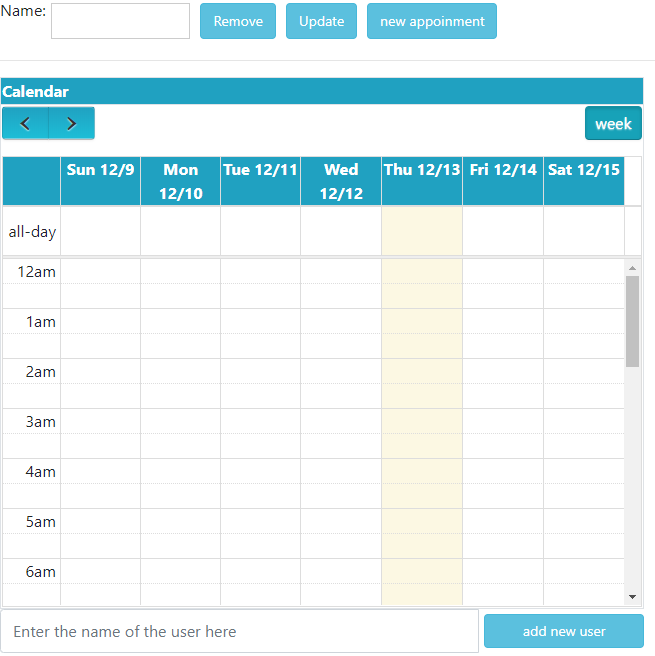
\includegraphics[width=0.9\linewidth]{images/screens/calendar1.png}}}%
    {\scriptsize%
     }
    \caption {A view at the interface of the Calendar App.}
    \label{fig:ev-fig-1}
\end{center}
\end{figure}

We can see the interface of the Calendar App at \figref*{fig:ev-fig-1}. As it was said, it provides the basic functionality, which every application of that sort should have: adding/removing users, creating appointmments from their behalf and editing this data. At the top left corner of the figure, we can observe a label \textit{Name:}, where there is a list of users on the right hand side from it. Apart from that, there is a calendar view, which covers the most space of the interface in the middle. Additionally, the functionality is controlled by four buttons: \textit{Remove} -- for removing selected users from the list of users; \textit{Update} -- for updating the available list of users and appointments from the server; \textit{new appointment} -- to create a new appointment on behalf of the selected user; \textit{add new participant} -- to add a participant with a name specified in the input on the left side from the button. 

Now, as we introduced our reader to the interface of the application and the functionality it has, we are going to demonstrate how a part of its functionality was integrated to work based on WebCure framework. 

In the original Calendar App, the feature of having users was implemented with Set CRDTs. Therefore, we extended the application to have our abstract \textit{SetCRDT} class on a client side, while also making the additional features of the application to work offline. For the demonstration purposes, we have the following setup: two separate Docker containers built on Antidote data store, interconnected for the mutual synchonisation; a configured server (according to the concepts introduced in WebCure) working with those two Antidote data stores; a web application that presents the view of two Calendar Apps simultaneously, while possessing all the offline features according to WebCure and a functionality to disconnect the link between two Antidote stores (mimicking network interruptions). 

\begin{figure}[!htb]
    \begin{center}
    \setlength{\fboxsep}{4pt}%
    \setlength{\fboxrule}{1pt}%
    \stackunder{\fbox{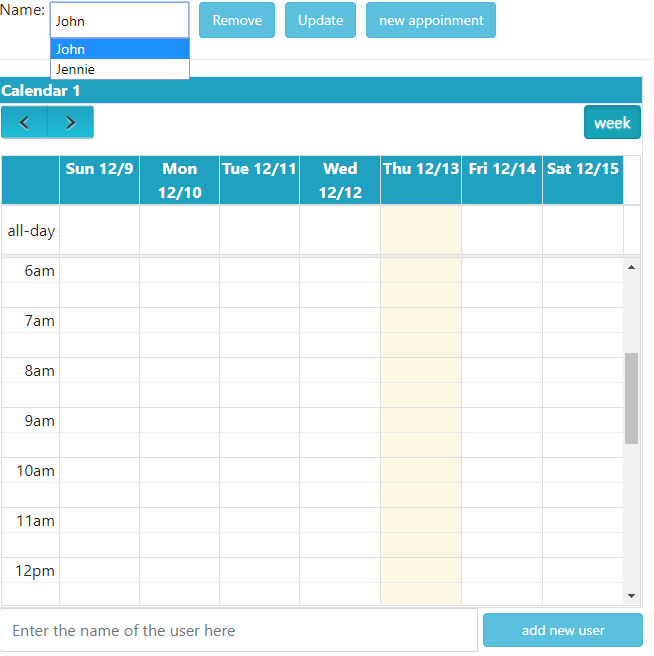
\includegraphics[width=0.9\linewidth]{images/screens/scr1.PNG}}}%
    {\scriptsize%
     }
    \caption {A view at the interface of the Calendar App.}
    \label{fig:ev-fig-2}
\end{center}
\end{figure}

\begin{lstlisting}[caption={The state of the users object store at the first Calendar App.}, label={lst:ev3}]
{
id: "users",
operations: [],
sentOperations: [],
state: Set(2) {"John", "Jennie"},
type: "set",
}
\end{lstlisting}

Let us say, we added two users with names \textit{John} and \textit{Jennie} to the first Calendar App, as \figref*{fig:ev-fig-2} shows. At this point, the first Calendar App will have its users stored under the \textit{``users''} id, as it is shown at \lstref*{lst:ev3}. The second Calendar App, at this point, will have its storage empty at client side, even though its server storage synchronizes with the server storage of the first Calendar. If the user of the second Calendar App requests the updates from its server by clicking the button \textit{Update}, the client storage of the second Calendar App would reach the same state as the first Calendar App has. However, for now, we are postponing this step.

Next, let us say, that we turn off the network for both calendar applications. Then, we firstly locally remove the user \textit{John} through the interface of the first Calendar App and, afterwards, we add a user \textit{Wayne} at the second Calendar App.

\begin{lstlisting}[caption={The state of the users object store after offline changes at the first Calendar App.}, label={lst:ev4}]
{
id: "users",
operations: [0: {type: "remove", value: "John"}],
sentOperations: [],
state: Set(2) {"John", "Jennie"},
type: "set"
}
\end{lstlisting}
\begin{lstlisting}[caption={The state of the users object store after offline changes at the second Calendar App.}, label={lst:ev5}]
{
id: "users",
operations: [0: {type: "add", value: "Wayne"}],
sentOperations: [],
state: Set(0) {},
type: "set"
}
\end{lstlisting}

As we are working offline, the changes will be applied straight away, so the local stores of the calendars will look like they are represented at \lstref*{lst:ev4} and \lstref*{lst:ev5}, respectively. As our reader observes, even thought both applications are in offline mode, they are still available and functional. 

\begin{lstlisting}[caption={The state of the users object store after the connection is enabled at the first Calendar App.}, label={lst:ev6}]
{
id: "users",
operations: [],
sentOperations: [0: {type: "remove", value: "John"}],
state: Set(2) {"John", "Jennie"},
type: "set"
}
\end{lstlisting}
\begin{lstlisting}[caption={The state of the users object store after the connection is enabled at the second Calendar App.}, label={lst:ev7}]
{
id: "users",
operations: [],
sentOperations: [0: {type: "add", value: "Wayne"}],
state: Set(0) {},
type: "set"
}
\end{lstlisting}

After we turn the connection back on, all the offline performed operations are sent to the server immediately. Therfefore, now the data stores of the calendars will change again. Basically, as we remember, the operations perfromed offline will move to the array \textit{sentOperations}. We can observe this behaviour at \lstref*{lst:ev6} and \lstref*{lst:ev7}.

\begin{lstlisting}[caption={The state of the users object store for both calendars.}, label={lst:ev8}]
{
id: "users",
operations: [],
sentOperations: [],
state: Set(2) {"Wayne", "Jennie"},
type: "set"
}
\end{lstlisting}

Finally, if the users request updates from the respective servers, associated with their applications, both calendars will reach the same state, as the servers converged having applied all the provided operations. At this point, at client sides of both Calendar Apps the state of the users local storage will look like it is shown at \lstref*{lst:ev8}.

\begin{figure}[!htb]
    \begin{center}
    \setlength{\fboxsep}{4pt}%
    \setlength{\fboxrule}{1pt}%
    \stackunder{\fbox{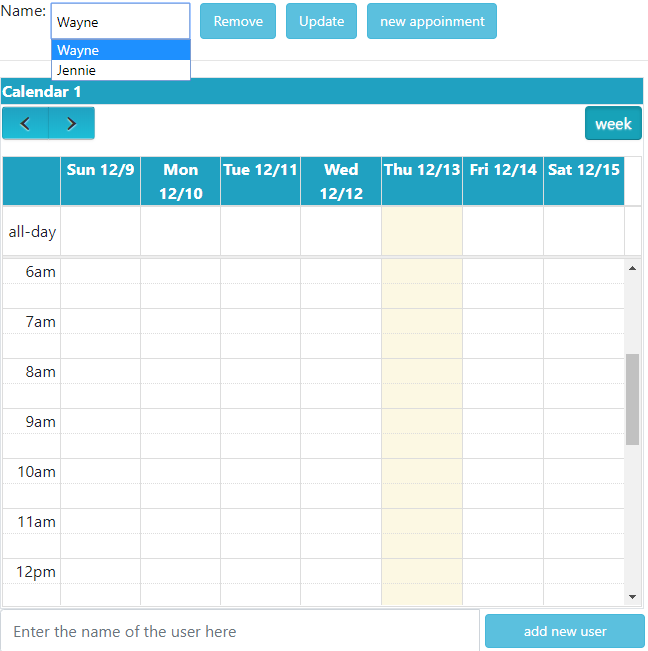
\includegraphics[width=0.9\linewidth]{images/screens/scr2.PNG}}}%
    {\scriptsize%
     }
    \caption {The final state of user list shown in the interface of the first Calendar (the same for the second one).}
    \label{fig:ev-fig-3}
\end{center}
\end{figure}

As we can see, the user \textit{John} was removed and the user \textit{Wayne} was added for both calendars. Obviously, all the operations took their effect in the interface as well, the final state of which is shown at \figref*{fig:ev-fig-3}.

To summarize this chapter, we took a working Calendar application and extended its functionality using the design concepts we developed for WebCure. The extended version proved to be available and functional offline and online, while partially replicating the data at client side, which lets users to continue working with their data. This example proves the point that WebCure allows to build applications based on it.